% !TEX program = lualatex
\documentclass[aspectratio=43,professionalfonts,handout]{beamer}
\usepackage{beamer_template}

\newcommand{\LectureNum}{18}
\newcommand{\LectureTitle}{三角関数のグラフ}
\newcommand{\TextPages}{p.\,149-151}
\newcommand{\NextTopic}{グラフの拡大と縮小（１）}
\newcommand{\NextPages}{p.\,152-154}
\newcommand{\CourseName}{基礎数学B}
\renewcommand{\TermName}{後期}

\begin{document}

% -----------------------------------------------
% スライド1: 表紙＋目標＋用語・定義
% -----------------------------------------------
\begin{frame}{\CourseName\quad 第\LectureNum 回「\LectureTitle 」}
  {\small \TermName\quad \TeacherName\quad ／\quad 教科書 \TextPages\quad
  \textbf{目標}：sin・cos・tan のグラフを描き、周期を理解できる}

  \begin{block}{用語・定義}
  \begin{description}[labelwidth=5.5em]
    \item[\kw{振幅}] ~
    \item[\kw{周期：y=sinx の周期は 2π}] ~
    \item[\kw{平行移動：y=sin(x-p)+q}] ~
  \end{description}
  \end{block}
\end{frame}

% -----------------------------------------------
% スライド2: 公式・性質
% -----------------------------------------------
\begin{frame}{公式・性質}
  \begin{block}{}
  \begin{itemize}
    \item y=sinx：振幅1、周期2π
    \item y=cosx：振幅1、周期2π
    \item y=tanx：周期π、x=π/2+nπ が漸近線
  \end{itemize}
  \end{block}
\end{frame}

% -----------------------------------------------
% スライド3: 図・グラフ（TikZコードを手動追加）
% -----------------------------------------------
\begin{frame}{図・グラフ}
  \centering
  % TODO: y=sinx・y=cosx・y=tanx の1周期分のグラフ比較
  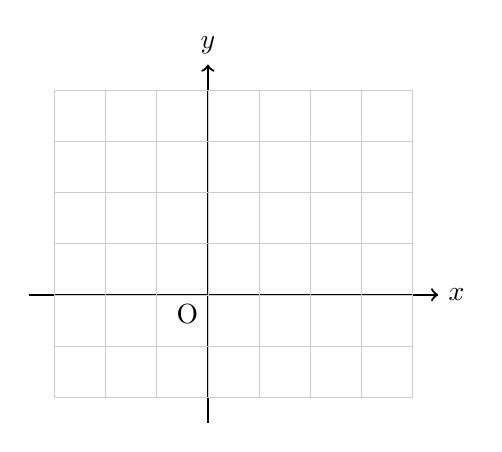
\begin{tikzpicture}[scale=0.65]
    \draw[->,thick] (-3.5,0) -- (4.5,0) node[right]{$x$};
    \draw[->,thick] (0,-2.5) -- (0,4.5) node[above]{$y$};
    \node[below left] at (0,0) {O};
    \draw[gray!40, very thin] (-3,-2) grid (4,4);
    % ここにグラフを描画
  \end{tikzpicture}
\end{frame}

% -----------------------------------------------
% スライド4: 例1→問1
% -----------------------------------------------
\begin{frame}{例1→問1}
  \begin{exampleblock}{例1) p.159（グラフをかけ・周期・振幅）}
    （板書で解説）
  \end{exampleblock}

  \vfill

  \begin{block}{問1) p.159\quad 自分で解いてみよう}
    （ノートに解くこと）
  \end{block}
\end{frame}

% -----------------------------------------------
% スライド5: 例2→問2
% -----------------------------------------------
\begin{frame}{例2→問2}
  \begin{exampleblock}{例2) p.160（平行移動したグラフ）}
    （板書で解説）
  \end{exampleblock}

  \vfill

  \begin{block}{問2) p.160\quad 自分で解いてみよう}
    （ノートに解くこと）
  \end{block}
\end{frame}

% -----------------------------------------------
% まとめ
% -----------------------------------------------
\begin{frame}{まとめ}
  \begin{itemize}
    \item % TODO: まとめを記入
  \end{itemize}

  \vfill
  {\small 基本問題：295, 296, 297}
\end{frame}

\end{document}
